\documentclass[11pt,a4paper]{article}

\usepackage[margin=2.3cm]{geometry}
\usepackage{amsmath,amssymb}
\usepackage{graphicx}
\usepackage{booktabs}
\usepackage{multirow}
\usepackage{array}
\usepackage{float}
\usepackage{caption}
\usepackage{subcaption}
\usepackage{xcolor}
\usepackage{listings}
\usepackage[hidelinks]{hyperref}

% ---------------------------------------------------------------
% Yellow boxes = parts the team still has to write.
% Delete every \TODO{...} before submitting.
% ---------------------------------------------------------------
\newcommand{\TODO}[1]{\par\smallskip\noindent\colorbox{yellow!35}{%
  \parbox{\dimexpr\linewidth-2\fboxsep}{\small\textbf{TODO:} #1}}\par\smallskip}

\lstset{language=Matlab, basicstyle=\ttfamily\footnotesize, numbers=left,
  numberstyle=\tiny\color{gray}, frame=single, breaklines=true,
  keywordstyle=\color{blue}, commentstyle=\color{green!50!black},
  stringstyle=\color{purple}, columns=fullflexible, showstringspaces=false}

% Tables are read with \tabinput (plain \input does not work inside tabular)
\makeatletter
\newcommand{\tabinput}[1]{\@@input #1 }
\makeatother

\newcommand{\FaVal}{-200{,}178}
\newcommand{\FbVal}{13{,}560}
\newcommand{\RootMaxDiff}{$7.24\times 10^{-7}$}
\newcommand{\BisFinalP}{2026.94122219}
\newcommand{\RuralSlope}{-98{,}067}
\newcommand{\UrbanSlope}{304{,}337}
\newcommand{\RuralChangeObs}{-4.06}
\newcommand{\UrbanChangeObs}{+17.34}


\title{\textbf{MATH 351 Numerical Methods with Applications}\\[4pt]
Group Project: Interpolation, Prediction and Root-Finding\\
for the Population of Kazakhstan}
\author{Student Name 1 \and Student Name 2 \and Student Name 3}
\date{Fall 2026}

\begin{document}
\maketitle

\TODO{Replace the student names above. Remove all yellow boxes before submitting.}

\tableofcontents
\newpage

% ===============================================================
\section{Introduction}
% ===============================================================
\TODO{Briefly describe the problem: predicting the population of Kazakhstan from a
few yearly values, why numerical interpolation and root-finding are useful here, and
what is done in each section of this report (5--8 sentences).}

Table~\ref{tab:data} shows the population data used in this project. All values
correspond to January~1 of each year.

\begin{table}[H]
\centering
\caption{Population of Kazakhstan on January 1.}
\label{tab:data}
\small
\begin{tabular}{lrrrrrr}
\toprule
Year & 2021 & 2022 & 2023 & 2024 & 2025 & 2026 \\
\midrule
All population   & 18{,}879{,}552 & 19{,}503{,}159 & 19{,}766{,}807 & 20{,}033{,}842 & 20{,}286{,}084 & 20{,}499{,}822 \\
Urban population & 11{,}151{,}376 & 11{,}991{,}238 & 12{,}209{,}896 & 12{,}451{,}192 & 12{,}774{,}743 & 13{,}085{,}110 \\
Rural population &  7{,}728{,}176 &  7{,}511{,}921 &  7{,}556{,}911 &  7{,}582{,}650 &  7{,}511{,}341 &  7{,}414{,}712 \\
\bottomrule
\end{tabular}
\end{table}

Throughout the report, time $t$ is measured in calendar years, so $t=2026$ means
January 1, 2026, and the fractional part of $t$ is the fraction of the year that has
passed.

% ===============================================================
\section{Numerical methods}
% ===============================================================
\TODO{Check that the descriptions below match what was taught in class, and add one
or two sentences in your own words for each method (main idea, advantages,
disadvantages).}

\subsection{Model 1: Lagrange interpolation polynomial}
Given $n+1$ distinct nodes $t_0,\dots,t_n$ with values $P_0,\dots,P_n$, the Lagrange
interpolation polynomial is the unique polynomial of degree at most $n$ with
$P(t_k)=P_k$:
\begin{equation}
P(t) = \sum_{k=0}^{n} P_k\, L_{n,k}(t), \qquad
L_{n,k}(t) = \prod_{\substack{i=0\\ i\neq k}}^{n} \frac{t-t_i}{t_k-t_i}.
\label{eq:lagrange}
\end{equation}
For Newton's method we also need its derivative, obtained from the product rule:
\begin{equation}
L_{n,k}'(t) = \sum_{\substack{j=0\\ j\neq k}}^{n} \frac{1}{t_k-t_j}
\prod_{\substack{i=0\\ i\neq k,\, i\neq j}}^{n} \frac{t-t_i}{t_k-t_i}.
\end{equation}

\subsection{Model 2: natural cubic spline}
On each subinterval $[t_j,t_{j+1}]$, $j=0,\dots,n-1$, the spline is a cubic polynomial
\begin{equation}
S_j(t) = a_j + b_j(t-t_j) + c_j(t-t_j)^2 + d_j(t-t_j)^3,
\end{equation}
such that $S$ interpolates the data and $S$, $S'$, $S''$ are continuous at the
interior nodes. The natural boundary conditions are $S''(t_0)=S''(t_n)=0$.
With $h_j = t_{j+1}-t_j$ and $a_j = P_j$, the coefficients $c_j$ solve the
tridiagonal system
\begin{equation}
h_{j-1}c_{j-1} + 2(h_{j-1}+h_j)c_j + h_j c_{j+1}
= \frac{3}{h_j}(a_{j+1}-a_j) - \frac{3}{h_{j-1}}(a_j-a_{j-1}),
\quad j=1,\dots,n-1,
\end{equation}
with $c_0=c_n=0$, and then
\begin{equation}
b_j = \frac{a_{j+1}-a_j}{h_j} - \frac{h_j}{3}(2c_j+c_{j+1}), \qquad
d_j = \frac{c_{j+1}-c_j}{3h_j}.
\end{equation}
For a prediction outside the data interval (e.g.\ $t=2026$ from data up to 2025)
the last cubic piece $S_{n-1}$ is used. Its derivative,
$S_j'(t) = b_j + 2c_j(t-t_j) + 3d_j(t-t_j)^2$, is used in Newton's method.

\subsection{Error and sensitivity measures}
\begin{equation}
E_{\text{abs}} = |P_{\text{actual}} - P_{\text{predicted}}|, \qquad
E_{\text{rel}} = \frac{|P_{\text{actual}} - P_{\text{predicted}}|}{|P_{\text{actual}}|}, \qquad
S = \frac{|P_{\text{perturbed}} - P_{\text{original}}|}{|P_{\text{original}}|}.
\end{equation}

\subsection{Root-finding methods}
We solve $F(t)=P(t)-20{,}700{,}000=0$.

\paragraph{Bisection.} Starting from $[a,b]$ with $F(a)F(b)<0$, set
$p=(a+b)/2$ and keep the half-interval where $F$ changes sign. After $n$ steps
$|t^*-p_n|\le (b-a)/2^{n+1}$, so the number of iterations for tolerance
$\mathrm{TOL}$ is known in advance:
$n=\lceil \log_2(b-a)-\log_2(2\,\mathrm{TOL})\rceil$.

\paragraph{Secant method.}
\begin{equation}
p_{k+1} = p_k - \frac{F(p_k)\,(p_k-p_{k-1})}{F(p_k)-F(p_{k-1})}.
\end{equation}

\paragraph{Newton's method.}
\begin{equation}
p_{k+1} = p_k - \frac{F(p_k)}{F'(p_k)}.
\end{equation}

For the secant and Newton methods we stop when $|p_k-p_{k-1}|<\mathrm{TOL}$.
The same tolerance $\mathrm{TOL}=10^{-6}$ years (about 30 seconds) is used for all
three methods.

% ===============================================================
\section{Task 1: Interpolation and prediction}
% ===============================================================
Both models were constructed from the 2021--2025 data and evaluated at $t=2026$.
The predictions are compared with the actual 2026 values in Table~\ref{tab:task1}
and plotted in Figure~\ref{fig:task1}.

\begin{table}[H]
\centering
\caption{Prediction of the 2026 population from the 2021--2025 data.}
\label{tab:task1}
\begin{tabular}{llrrrr}
\toprule
Category & Model & Predicted 2026 & Actual 2026 & $E_{\text{abs}}$ & $E_{\text{rel}}$ \\
\midrule
\tabinput{tables/task1.tex}
\bottomrule
\end{tabular}
\end{table}

\begin{figure}[H]
\centering
\begin{subfigure}{0.49\textwidth}
  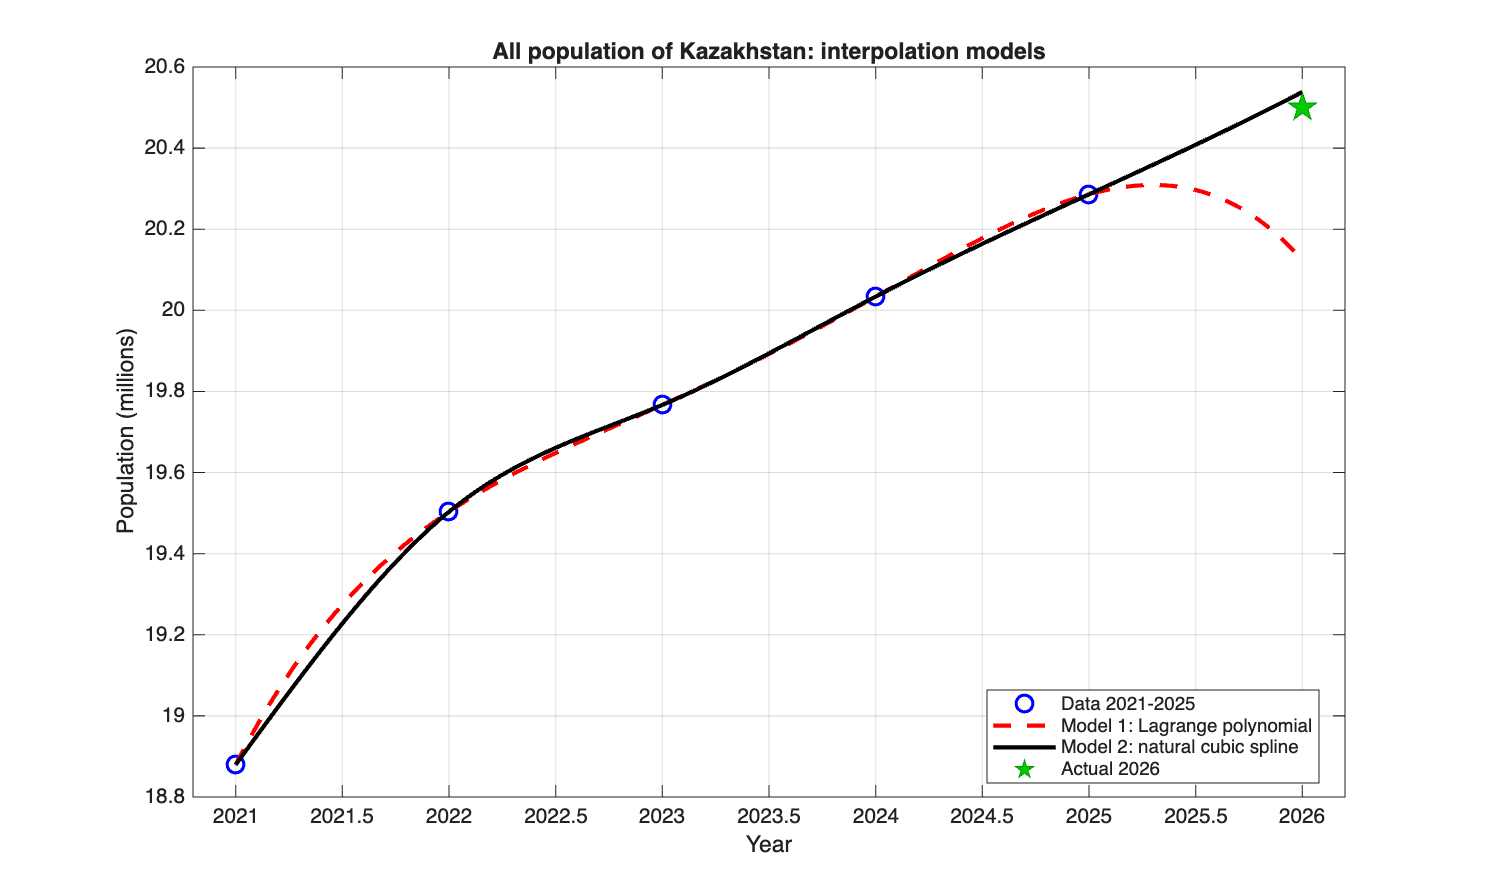
\includegraphics[width=\linewidth]{figures/task1_all.png}
  \caption{All population}
\end{subfigure}
\hfill
\begin{subfigure}{0.49\textwidth}
  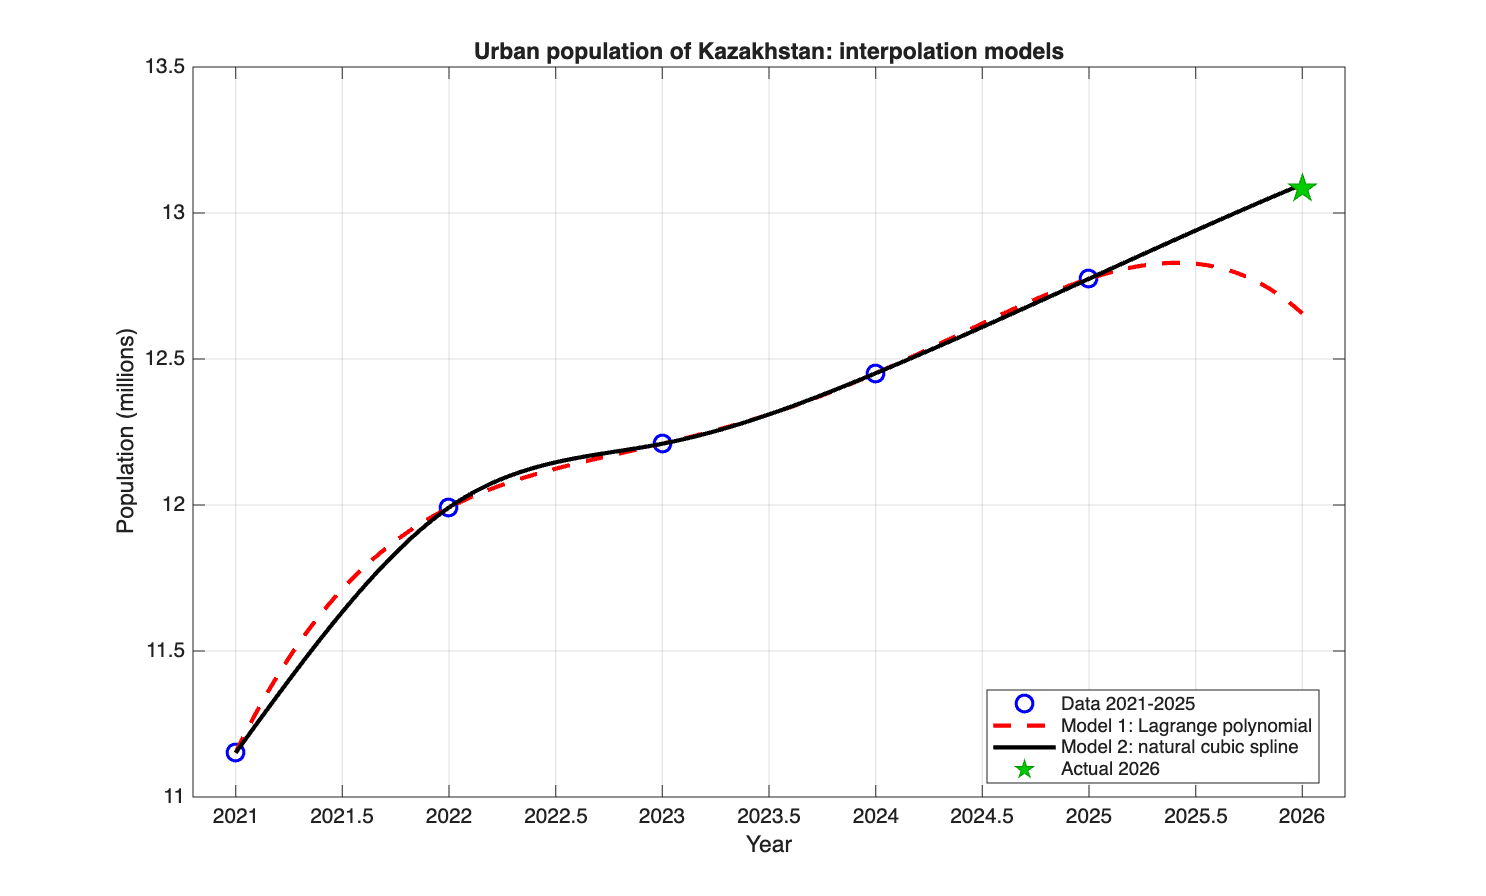
\includegraphics[width=\linewidth]{figures/task1_urban.png}
  \caption{Urban population}
\end{subfigure}

\medskip
\begin{subfigure}{0.49\textwidth}
  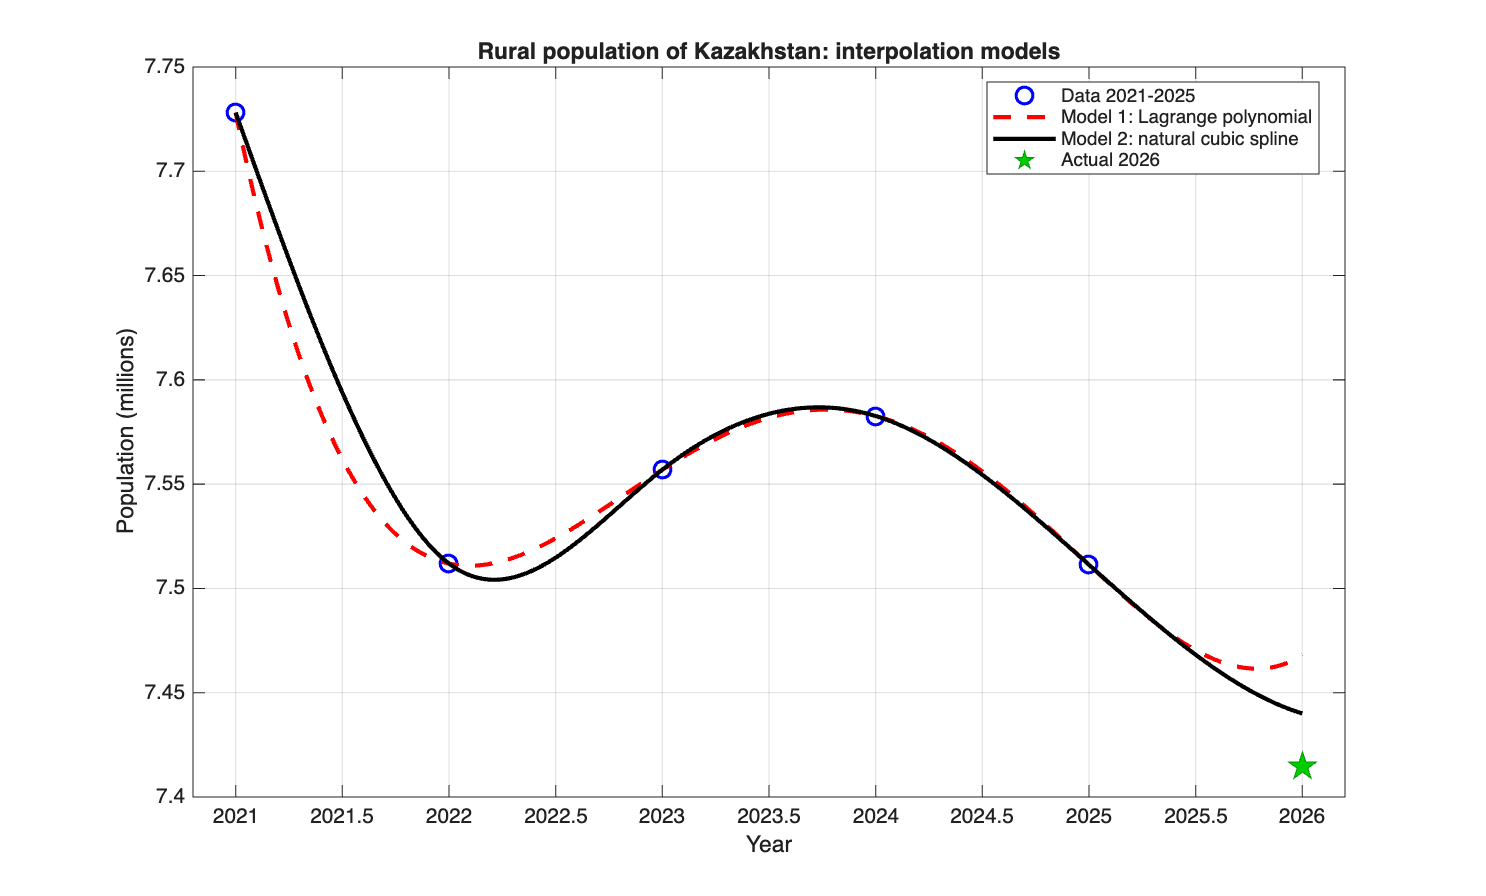
\includegraphics[width=\linewidth]{figures/task1_rural.png}
  \caption{Rural population}
\end{subfigure}
\caption{Lagrange polynomial (dashed) and natural cubic spline (solid) built on the
2021--2025 data (circles), plotted over 2021--2026. The star is the actual 2026
value.}
\label{fig:task1}
\end{figure}

\TODO{Compare the two models (3--5 sentences). Points you can use: the spline is
closer to the actual 2026 value in all three categories; the Lagrange polynomial
bends away after 2025 (see the figure), especially for the all and urban
population; relative errors are given in Table~\ref{tab:task1}.}

% ===============================================================
\section{Task 2: Model validation and error analysis}
% ===============================================================
Each model was built on the data up to year $m$ and used to predict year $m+1$,
for $m=2023,2024,2025$. The results are given in
Tables~\ref{tab:task2all}--\ref{tab:task2summary}.

\newcommand{\backtesthead}{%
Data used & Target & Actual &
\multicolumn{3}{c}{Model 1: Lagrange} & \multicolumn{3}{c}{Model 2: Spline} \\
\cmidrule(lr){4-6}\cmidrule(lr){7-9}
 & & & Predicted & $E_{\text{abs}}$ & $E_{\text{rel}}$ & Predicted & $E_{\text{abs}}$ & $E_{\text{rel}}$ \\}

\begin{table}[H]
\centering
\caption{Back-testing results: all population.}
\label{tab:task2all}
\resizebox{\textwidth}{!}{%
\begin{tabular}{llrrrrrrr}
\toprule
\backtesthead
\midrule
\tabinput{tables/task2_all.tex}
\bottomrule
\end{tabular}}
\end{table}

\begin{table}[H]
\centering
\caption{Back-testing results: urban population.}
\label{tab:task2urban}
\resizebox{\textwidth}{!}{%
\begin{tabular}{llrrrrrrr}
\toprule
\backtesthead
\midrule
\tabinput{tables/task2_urban.tex}
\bottomrule
\end{tabular}}
\end{table}

\begin{table}[H]
\centering
\caption{Back-testing results: rural population.}
\label{tab:task2rural}
\resizebox{\textwidth}{!}{%
\begin{tabular}{llrrrrrrr}
\toprule
\backtesthead
\midrule
\tabinput{tables/task2_rural.tex}
\bottomrule
\end{tabular}}
\end{table}

\begin{table}[H]
\centering
\caption{Summary of the back-testing: mean relative error over the three
predictions, and the number of predictions in which each model had the smaller
error.}
\label{tab:task2summary}
\begin{tabular}{lrrcc}
\toprule
Category & Mean $E_{\text{rel}}$ Lagrange & Mean $E_{\text{rel}}$ Spline & Lagrange better & Spline better \\
\midrule
\tabinput{tables/task2_summary.tex}
\bottomrule
\end{tabular}
\end{table}

\subsection*{Discussion}
\TODO{(a) Which model gives the smaller prediction errors? Use Table~\ref{tab:task2summary}.}
\TODO{(b) Is the same model consistently better for all categories and all years?
Look at each row of Tables~\ref{tab:task2all}--\ref{tab:task2rural}. Note that even
the spline's error is not always small: e.g.\ the rural 2025 prediction.}
\TODO{(c) Is it reasonable to choose a model based on only one prediction? Explain
(e.g.\ one year can be lucky or unlucky; errors change from year to year).}

% ===============================================================
\section{Task 3: Sensitivity and stability}
% ===============================================================
The 2024 value was changed by $0.5\%$, both models were rebuilt on the 2021--2025
data, and the 2026 predictions before and after the change were compared
(Table~\ref{tab:task3}). The column $S/0.005$ shows how many times the relative
change of the prediction is larger than the relative change made in the data.

\begin{table}[H]
\centering
\caption{Sensitivity of the 2026 prediction to a $0.5\%$ change in the 2024 value.}
\label{tab:task3}
\resizebox{\textwidth}{!}{%
\begin{tabular}{llrrrrc}
\toprule
Experiment & Model & $P_{\text{original}}$ & $P_{\text{perturbed}}$ & $S$ & $S/0.005$ &
$S_{\text{Lagrange}}/S_{\text{Spline}}$ \\
\midrule
\tabinput{tables/task3.tex}
\bottomrule
\end{tabular}}
\end{table}

\subsection*{Discussion}
\TODO{Which model is more stable with respect to small changes in the data?
(The Lagrange prediction changes by about $5\%$, i.e.\ about 10 times the data
change; the spline changes by about $0.5\%$.)}
\TODO{Must a model that interpolates all data points exactly give a reliable
prediction? (Both models pass through every data point, yet their predictions
differ a lot.)}
\TODO{Which model do you select for Tasks 4, 6 and 7, and why? Refer to both Task 2
and Task 3. (The code uses the natural cubic spline.)}

% ===============================================================
\section{Task 4: Population threshold and root-finding}
% ===============================================================
The selected model (natural cubic spline) was built on the total population data
for 2023--2026. The equation
\[
F(t) = P(t) - 20{,}700{,}000 = 0
\]
was solved by the three methods. Since $F(2026)=\FaVal<0$ and
$F(2027)=\FbVal>0$, the root lies in $[2026,2027]$. The settings were:
\begin{itemize}
  \item Bisection: initial interval $[a,b]=[2026,2027]$;
  \item Secant: initial approximations $p_0=2026$, $p_1=2027$;
  \item Newton: initial approximation $p_0=2026$;
  \item stopping tolerance $\mathrm{TOL}=10^{-6}$ years for all methods.
\end{itemize}

\begin{table}[H]
\centering
\caption{Bisection method iterations.}
\label{tab:bisection}
\small
\begin{tabular}{rrrrr}
\toprule
$k$ & $a_k$ & $b_k$ & $p_k$ & $F(p_k)$ \\
\midrule
\tabinput{tables/task4_bisection.tex}
\bottomrule
\end{tabular}
\end{table}
The final bisection approximation is the midpoint of the last interval,
$p=\BisFinalP$.

\begin{table}[H]
\centering
\caption{Secant method iterations.}
\label{tab:secant}
\begin{tabular}{rrrr}
\toprule
$i$ & $p_i$ & $F(p_i)$ & $|p_i-p_{i-1}|$ \\
\midrule
\tabinput{tables/task4_secant.tex}
\bottomrule
\end{tabular}
\end{table}

\begin{table}[H]
\centering
\caption{Newton's method iterations.}
\label{tab:newton}
\begin{tabular}{rrrr}
\toprule
$i$ & $p_i$ & $F(p_i)$ & $|p_i-p_{i-1}|$ \\
\midrule
\tabinput{tables/task4_newton.tex}
\bottomrule
\end{tabular}
\end{table}

\begin{table}[H]
\centering
\caption{Comparison of the three root-finding methods.}
\label{tab:task4summary}
\begin{tabular}{lrcccl}
\toprule
Method & Root $t^*$ & Iterations & $F$ evaluations & $F'$ evaluations & Predicted date \\
\midrule
\tabinput{tables/task4_summary.tex}
\bottomrule
\end{tabular}
\end{table}

\begin{figure}[H]
\centering
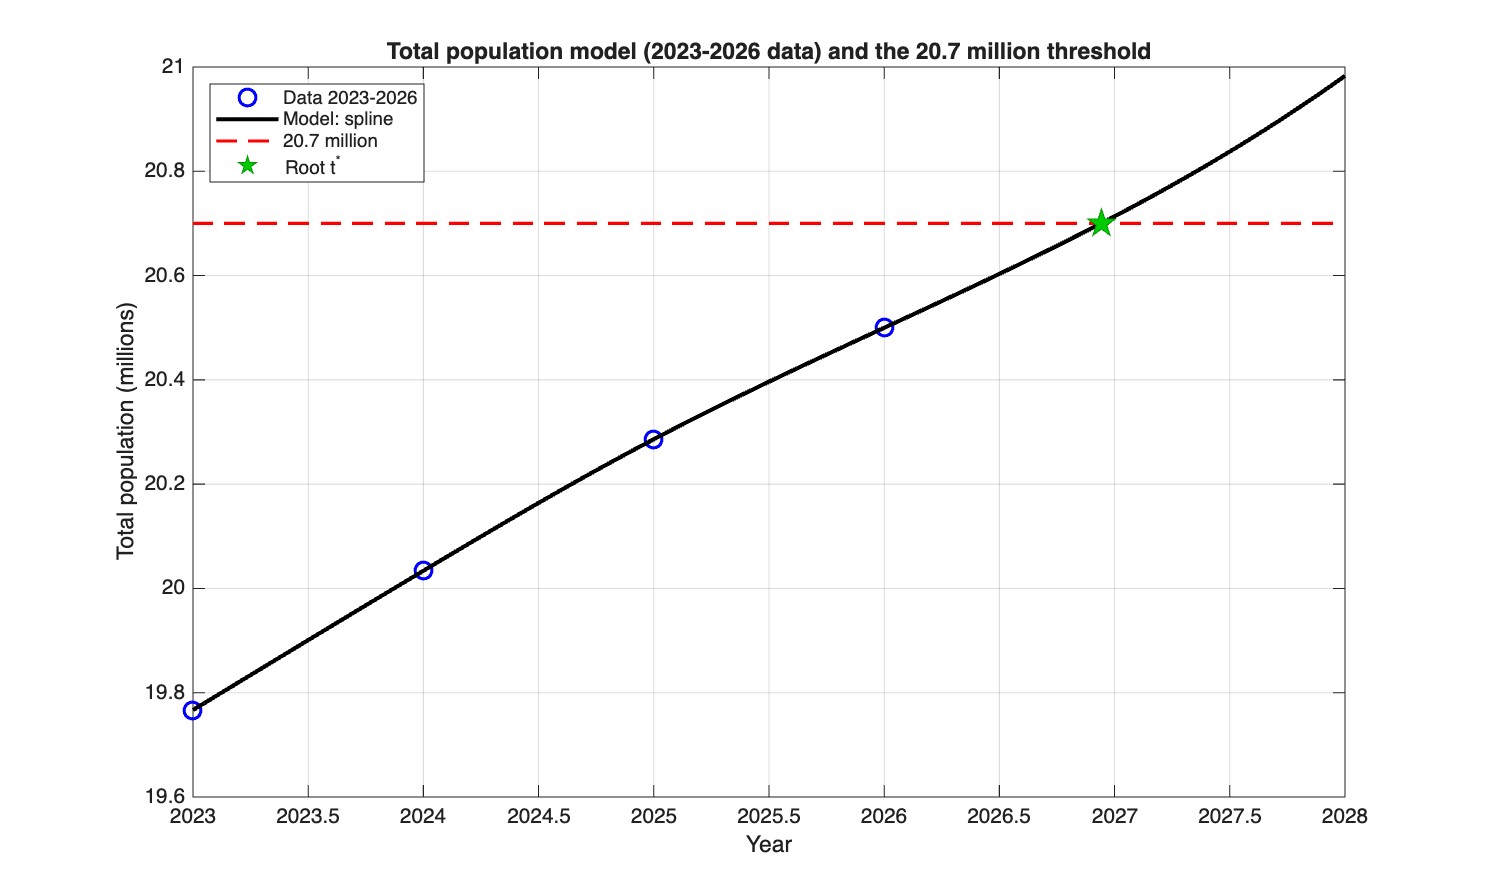
\includegraphics[width=0.7\textwidth]{figures/task4_threshold.png}
\caption{Natural cubic spline for the total population (2023--2026 data) and the
20.7 million threshold. The star marks the computed root $t^*$.}
\label{fig:task4}
\end{figure}

\subsection*{Discussion}
\TODO{Compare convergence, computational effort and reliability of the three
methods (Table~\ref{tab:task4summary}). Bisection: guaranteed to converge, but
slow (linear, error halves each step). Secant: no derivative needed, fast
(superlinear). Newton: fastest (quadratic, see how $|p_i-p_{i-1}|$ drops in
Table~\ref{tab:newton}), but needs $F'$ and a good starting point.}
\TODO{Do the three methods give essentially the same answer? (Yes: they differ by
at most \RootMaxDiff{} years.) Does that mean they are equally efficient? Explain
using the number of iterations and function evaluations.}

% ===============================================================
\section{Task 5: Alternative methods for population prediction}
% ===============================================================
\TODO{At least 300 words. Find at least two peer-reviewed journal papers on
population prediction or forecasting (e.g.\ logistic growth models, ARIMA time
series, cohort-component method, machine learning). For each approach: main idea,
comparison with interpolation, advantages and disadvantages. State your preferred
model and refer to numerical results from Tasks 1--4 (e.g.\ back-testing errors,
sensitivity factor $\approx 10$ for Lagrange). Add the papers to the reference list.}

% ===============================================================
\section{Task 6: Rural population, prediction and interpretation}
% ===============================================================
Using the natural cubic spline built on all data from 2021--2026, the rural
population was projected to 2028 and 2030 (Table~\ref{tab:task6},
Figure~\ref{fig:task6}). For comparison, the Lagrange polynomial built on the
same data is also shown.

\begin{table}[H]
\centering
\caption{Projected rural population.}
\label{tab:task6}
\begin{tabular}{lrrrr}
\toprule
Year & Spline projection & Change vs.\ 2026 & Change (\%) & Lagrange (comparison) \\
\midrule
\tabinput{tables/task6_rural.tex}
\bottomrule
\end{tabular}
\end{table}

\begin{figure}[H]
\centering
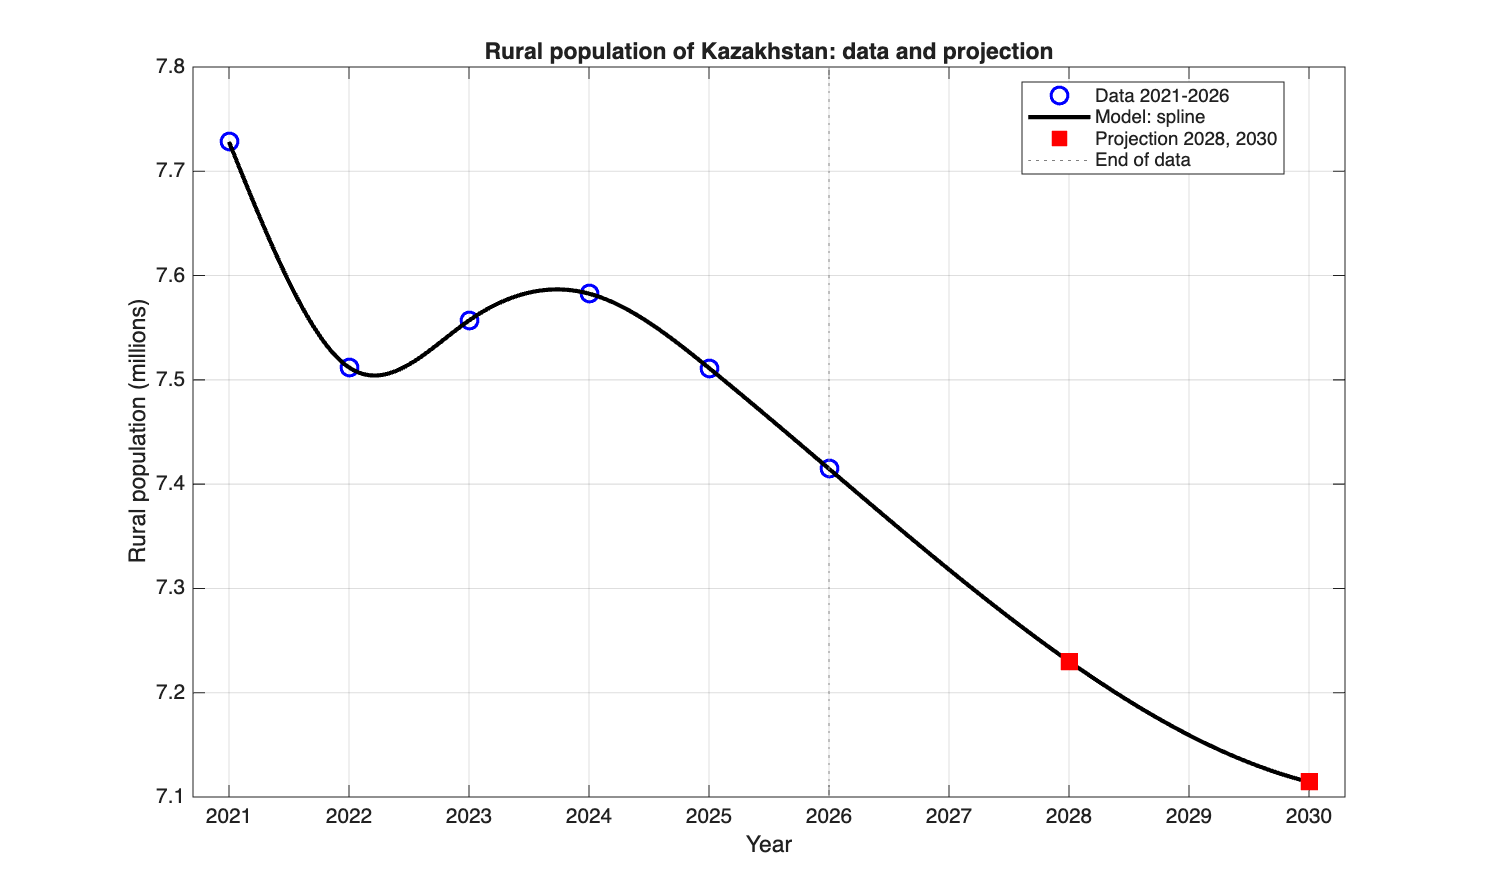
\includegraphics[width=0.7\textwidth]{figures/task6_rural.png}
\caption{Rural population: data 2021--2026 (circles), natural cubic spline and the
projections for 2028 and 2030 (squares).}
\label{fig:task6}
\end{figure}

\TODO{At least 200 words. Trend (rural population fell by
$\RuralChangeObs\%$ from 2021 to 2026; slope of the spline at 2026 is
$\RuralSlope$ people per year); reliability of the 2028 and 2030 predictions
(use the back-testing error, e.g.\ rural 2025 relative error of the spline, and the
sensitivity result); limitations of long-term extrapolation (note the very different
Lagrange values); actions or investments that could influence rural areas.}

% ===============================================================
\section{Task 7: Urban population, prediction and interpretation}
% ===============================================================
Using the natural cubic spline built on all data from 2021--2026, the urban
population was projected to 2028 and 2030 (Table~\ref{tab:task7},
Figure~\ref{fig:task7}).

\begin{table}[H]
\centering
\caption{Projected urban population.}
\label{tab:task7}
\begin{tabular}{lrrrr}
\toprule
Year & Spline projection & Change vs.\ 2026 & Change (\%) & Lagrange (comparison) \\
\midrule
\tabinput{tables/task7_urban.tex}
\bottomrule
\end{tabular}
\end{table}

\begin{figure}[H]
\centering
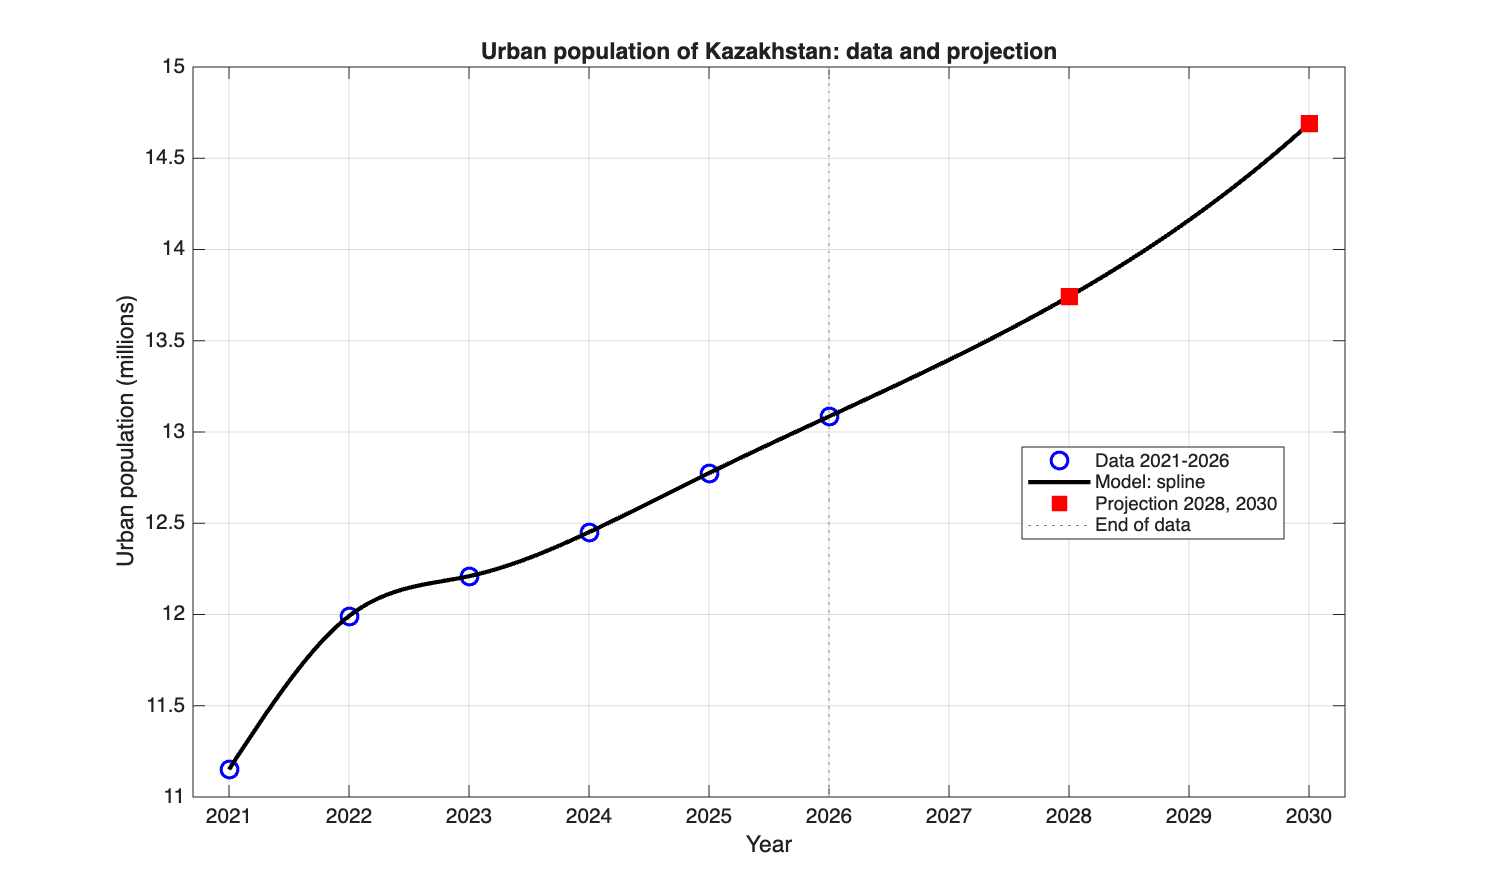
\includegraphics[width=0.7\textwidth]{figures/task7_urban.png}
\caption{Urban population: data 2021--2026 (circles), natural cubic spline and the
projections for 2028 and 2030 (squares).}
\label{fig:task7}
\end{figure}

\TODO{At least 200 words. Trend (urban population grew by
$\UrbanChangeObs\%$ from 2021 to 2026; slope at 2026 is $\UrbanSlope$ people per
year); reliability of the predictions (back-testing and sensitivity numbers);
limitations of extrapolation (the Lagrange value for 2030 is clearly unrealistic);
opportunities and challenges of urban growth; which areas you would prioritize as an
investor or decision-maker.}

% ===============================================================
\section{MATLAB implementation}
% ===============================================================
The complete code is submitted separately; \texttt{main.m} runs all tasks. The
methods are based on the MATLAB codes from the lecture slides (Lecture~3: bisection;
Lecture~4: natural cubic spline). The modifications made for this project are
shown below.

\TODO{Explain each excerpt in your own words: what was changed compared to the
lecture code, and why.}

\paragraph{Spline evaluation outside the data range.}
The lecture function \texttt{natural\_spline} searches for the subinterval that
contains the query point, so it cannot be evaluated after the last data year. We
added \texttt{spline\_piece}, which uses the last (or first) cubic piece outside
the data range.
\lstinputlisting[firstline=13,lastline=19]{code/natural_spline.m}
\lstinputlisting{code/spline_piece.m}

\paragraph{Bisection with an iteration table.}
The lecture algorithm is unchanged; each iteration is stored in \texttt{hist} so
that Table~\ref{tab:bisection} can be printed.
\lstinputlisting[firstline=10,lastline=28]{code/bisect.m}

\paragraph{Newton's and secant methods.}
These are written from the lecture pseudocode (Algorithm~2.3 and the secant
formula), with the stopping rule $|p_i-p_{i-1}|<\mathrm{TOL}$.
\lstinputlisting[firstline=4,lastline=21]{code/newton.m}
\lstinputlisting[firstline=4,lastline=23]{code/secant.m}

\paragraph{Lagrange interpolation.}
Written directly from formula~\eqref{eq:lagrange}.
\lstinputlisting{code/LagrangeInterpolation.m}

% ===============================================================
\section{Conclusion}
% ===============================================================
\TODO{Short summary (5--8 sentences): which model was better and why (back-testing
and sensitivity numbers), when the population reaches 20.7 million (December 2026),
the main projections for 2028 and 2030, and the main limitation of interpolation for
long-term prediction.}

% ===============================================================
\begin{thebibliography}{9}
% ===============================================================
\bibitem{lectures} Y.~Amanbek, \emph{MATH 351 Numerical Methods with Applications},
lecture slides, Chapters 3 and 4, Nazarbayev University, Fall 2026.
\bibitem{burden} R.~L.~Burden, J.~D.~Faires, A.~M.~Burden, \emph{Numerical Analysis},
10th ed., Cengage Learning, 2016.
\bibitem{paper1} \TODO{Peer-reviewed paper 1 (authors, title, journal, volume, pages, year, DOI).}
\bibitem{paper2} \TODO{Peer-reviewed paper 2 (authors, title, journal, volume, pages, year, DOI).}
\end{thebibliography}

\end{document}
